\chapter{Evaluation}
\label{cha:eval}
In this chapter, the intersection of the inventor-patent instance dataset from the Flemming's research and the engineer and scientist (E\&S) inventor-patent instance dataset from the work done by Chunmian et al is used to evaluate the performance of my approach.  In section 5.1, the details of the datasets are introduced. In section 5.2, the measurements of the performance of my approach are described. Finally, the evaluation result is discussed in the section 5.3. 

\section{Datasets}
The dataset used for the evaluation is the intersection of the inventor-patent instance dataset from the Flemming's work and the the engineer and scientist (E\&S) dataset from the work done by Chunmian et al. The Flemming's dataset contains the inventor-patent instances from USPTO of the period from 1975 to 2010. This inventor-patent instances have been preprocessed by the Flemming's approach. The Flemming's dataset provides some useful information for the inventor-patent instances such as the patent assignee number, the longitude and the latitude which cannot be extracted from the patent documents. The E\&S dataset contains the inventor identification information for each inventor of the inventor-patent instance.  The intersection set of the two datasets contains 32495 inventor-patent instances. The patent texts are extracted by using the patent full-text search engine developed by the USPTO.  The publication information is extracted from the Europe PMC by using its search engine. Another benchmark dataset \cite{RePEc:eee:respol:v:43:y:2014:i:6:p:941-955} used by Flemming for the evaluation is also used to compare my approach with the Flemming's. Because the publication database used for the evaluation is the Europe PMC which only contains the bio-medical publications, the subset of the intersection dataset which contains the inventor-patent instances from the biomedical field is used to evaluate the patent-publication matching performance. This subset contains 3604 inventor-patent instances. 

\section{Measurements}
There are five measurements to evaluate the accuracy of my approach for the inventor identification. They are "F-measure" or "F-Score", "lumping error" , "splitting error", "precision" and "recall". In order to calculate these measurements, four basic values should be calculated first based on the clustering result. They are true positive, false positive, true negative and false negative.  After the clustering, each cluster contains some instances which are hoped to have the same inventor ID. The dataset for the evaluation assigns each instance an inventor ID as the true value.  Within one cluster, the pairs of the instances with the same IDs are considered to be correct and the other pairs are considered to be incorrect. For different clusters, the pairs of the instances with different IDs are considered to be correct and the others are considered to be incorrect. The table 5.1 shows how to calculate the four basic values based on the numbers of the correct pairs and the incorrect pairs.
\begin{table}
\centering
\begin{tabular}{|c|c|c|}
\hline
 & Same Cluster & Different Clusers \\
 \hline
 Same ID & True Positive(TP) & False Negative(FN)  \\
 \hline
Different IDs & False Positive(FP) & True Negative(TN) \\
\hline
\end{tabular}
\caption{Four Basic Values For the Evaluation}
\end{table}
After calculating the four basic values, the \emph{precision} and the \emph{recall} are calculated and the \emph{F-measure} is calculated based on the \emph{precision} and the \emph{recall}. 
\begin{equation}
Precision =\frac{TP}{TP+FP}
\end{equation} 
\begin{equation}
Recall =\frac{TP}{TP+FN}
\end{equation} 
\begin{equation}
F-measure= \frac{2}{\frac{1}{Precision}+\frac{1}{Recall}}
\end{equation}
The \emph{precision} represents the fraction of the inventor-patent instances which have the same inventor IDs in all the clusters and the \emph{recall} represents the fraction of the inventor-patent instances which have the same IDs have been put correctly in the same clusters. The \emph{F-measure} is the harmonic mean of the \emph{precision} and the \emph{recall} which considers both the \emph{precision} and the \emph{recall}. It is the main measurement to evaluate the performance.  The four basic values can also be used to compute another two values: the \emph{lumping} error and the \emph{splitting} error.
\begin{equation}
Lumping=\frac{FP}{TP+FN}
\end{equation}
\begin{equation}
Splitting=\frac{FN}{TP+FN}
\end{equation}
The \emph{lumping} error occurs when the instances from different inventors are grouped in the same cluster while the \emph{splitting} error occurs when the instances from the same person are put into different clusters. Flemming points out the \emph{lumping} error and the \emph{splitting} error are more intuitive and they are negatively correlated \cite{RePEc:eee:respol:v:43:y:2014:i:6:p:941-955}. From the definition, a good result for the inventor identification should have the small values for the \emph{lumping} error and the \emph{splitting} error and high values for the \emph{F-measure}, the \emph{precision} and the \emph{recall}.

\section{Evaluation}
The machine used for the evaluation is Mac-mini with the Mac-OS operating system. The CPU is Intel Core i5 (3M Cache, up to 2.6GHz). The RAM is 8GB. The evaluation for my thesis approach is divided into 5 parts. The intersection of the inventor-patent instance datasets is divided into two datasets, the training dataset and the testing dataset. The training dataset randomly picks 8000 instances from the intersection of the inventor-patent instance datasets. The rest of the intersection is used as the testing dataset. The first part uses these 8000 instances to do the training and the cross-validation for the logistic regression with the clustering. The second part randomly picks 5000 instances from the testing dataset to test the transitivity effect on the clustering result. The third part is to test the clustering performance on the testing dataset by using the values of the parameters from the first part of the evaluation. The fourth part compares my approach with the Flemming's approach by using the benchmark dataset. The last part of the evaluation tests the patent-publication matching effect on the clustering result.

\subsection{the Cross Validation for Logistic Regression with Clustering}
In the first part of the evaluation, the training inventor-patent instance dataset which contains 8000 instances is used for the cross validation. For each time, subsets with different sizes are randomly extracted from the training dataset. A 5-folder cross validation is performed on the extracted subset of the dataset. For each iteration of the cross validation, a logistic regression is performed first to generate the weights and the threshold. The weights and the threshold are used by the hierarchical clustering and the DBSCAN. The five measurements are calculated for the clustering result. For different sizes of the subsets, the standard errors and the mean values of the five measurements are also calculated to test the stability of the logistic regression with the clustering. The size of the subset of the training data changes from 2000 to 8000 and the increment is 2000. The hierarchical clustering uses the single linkage clustering method and the minPts of the DBSCAN is 1.
\newline

The figure 5.1 and the figure 5.2 show the mean values of measurement plots with respect to the subset size for the hierarchical clustering and the DBSCAN separately. From the plots, the points in the plots represent the mean values for the measurements and the lines represent the two times of the standard errors of the measurements. From the result of the cross validation, the single linkage clustering have the exactly same result as the DBSCAN with minPts of 1. The reason is that both of them result in a chain rule \footnote{Chain Rule: If A is similar to B and B is similar to C, A is similar to C.} for the inventor identity. The \emph{F-measure}, the \emph{precision} and the \emph{recall} are all more than 0.99 and the standard errors are less than 0.01. The \emph{lumping} error and the \emph{splitting} error are both less than 0.01 and the standard errors are also less than 0.01. From the figure 5.1 and the figure 5.2, the logistic regression with the clustering is stable. They also show good performance of the clustering result for the inventor identification.  \newline

\begin{figure}
\centering
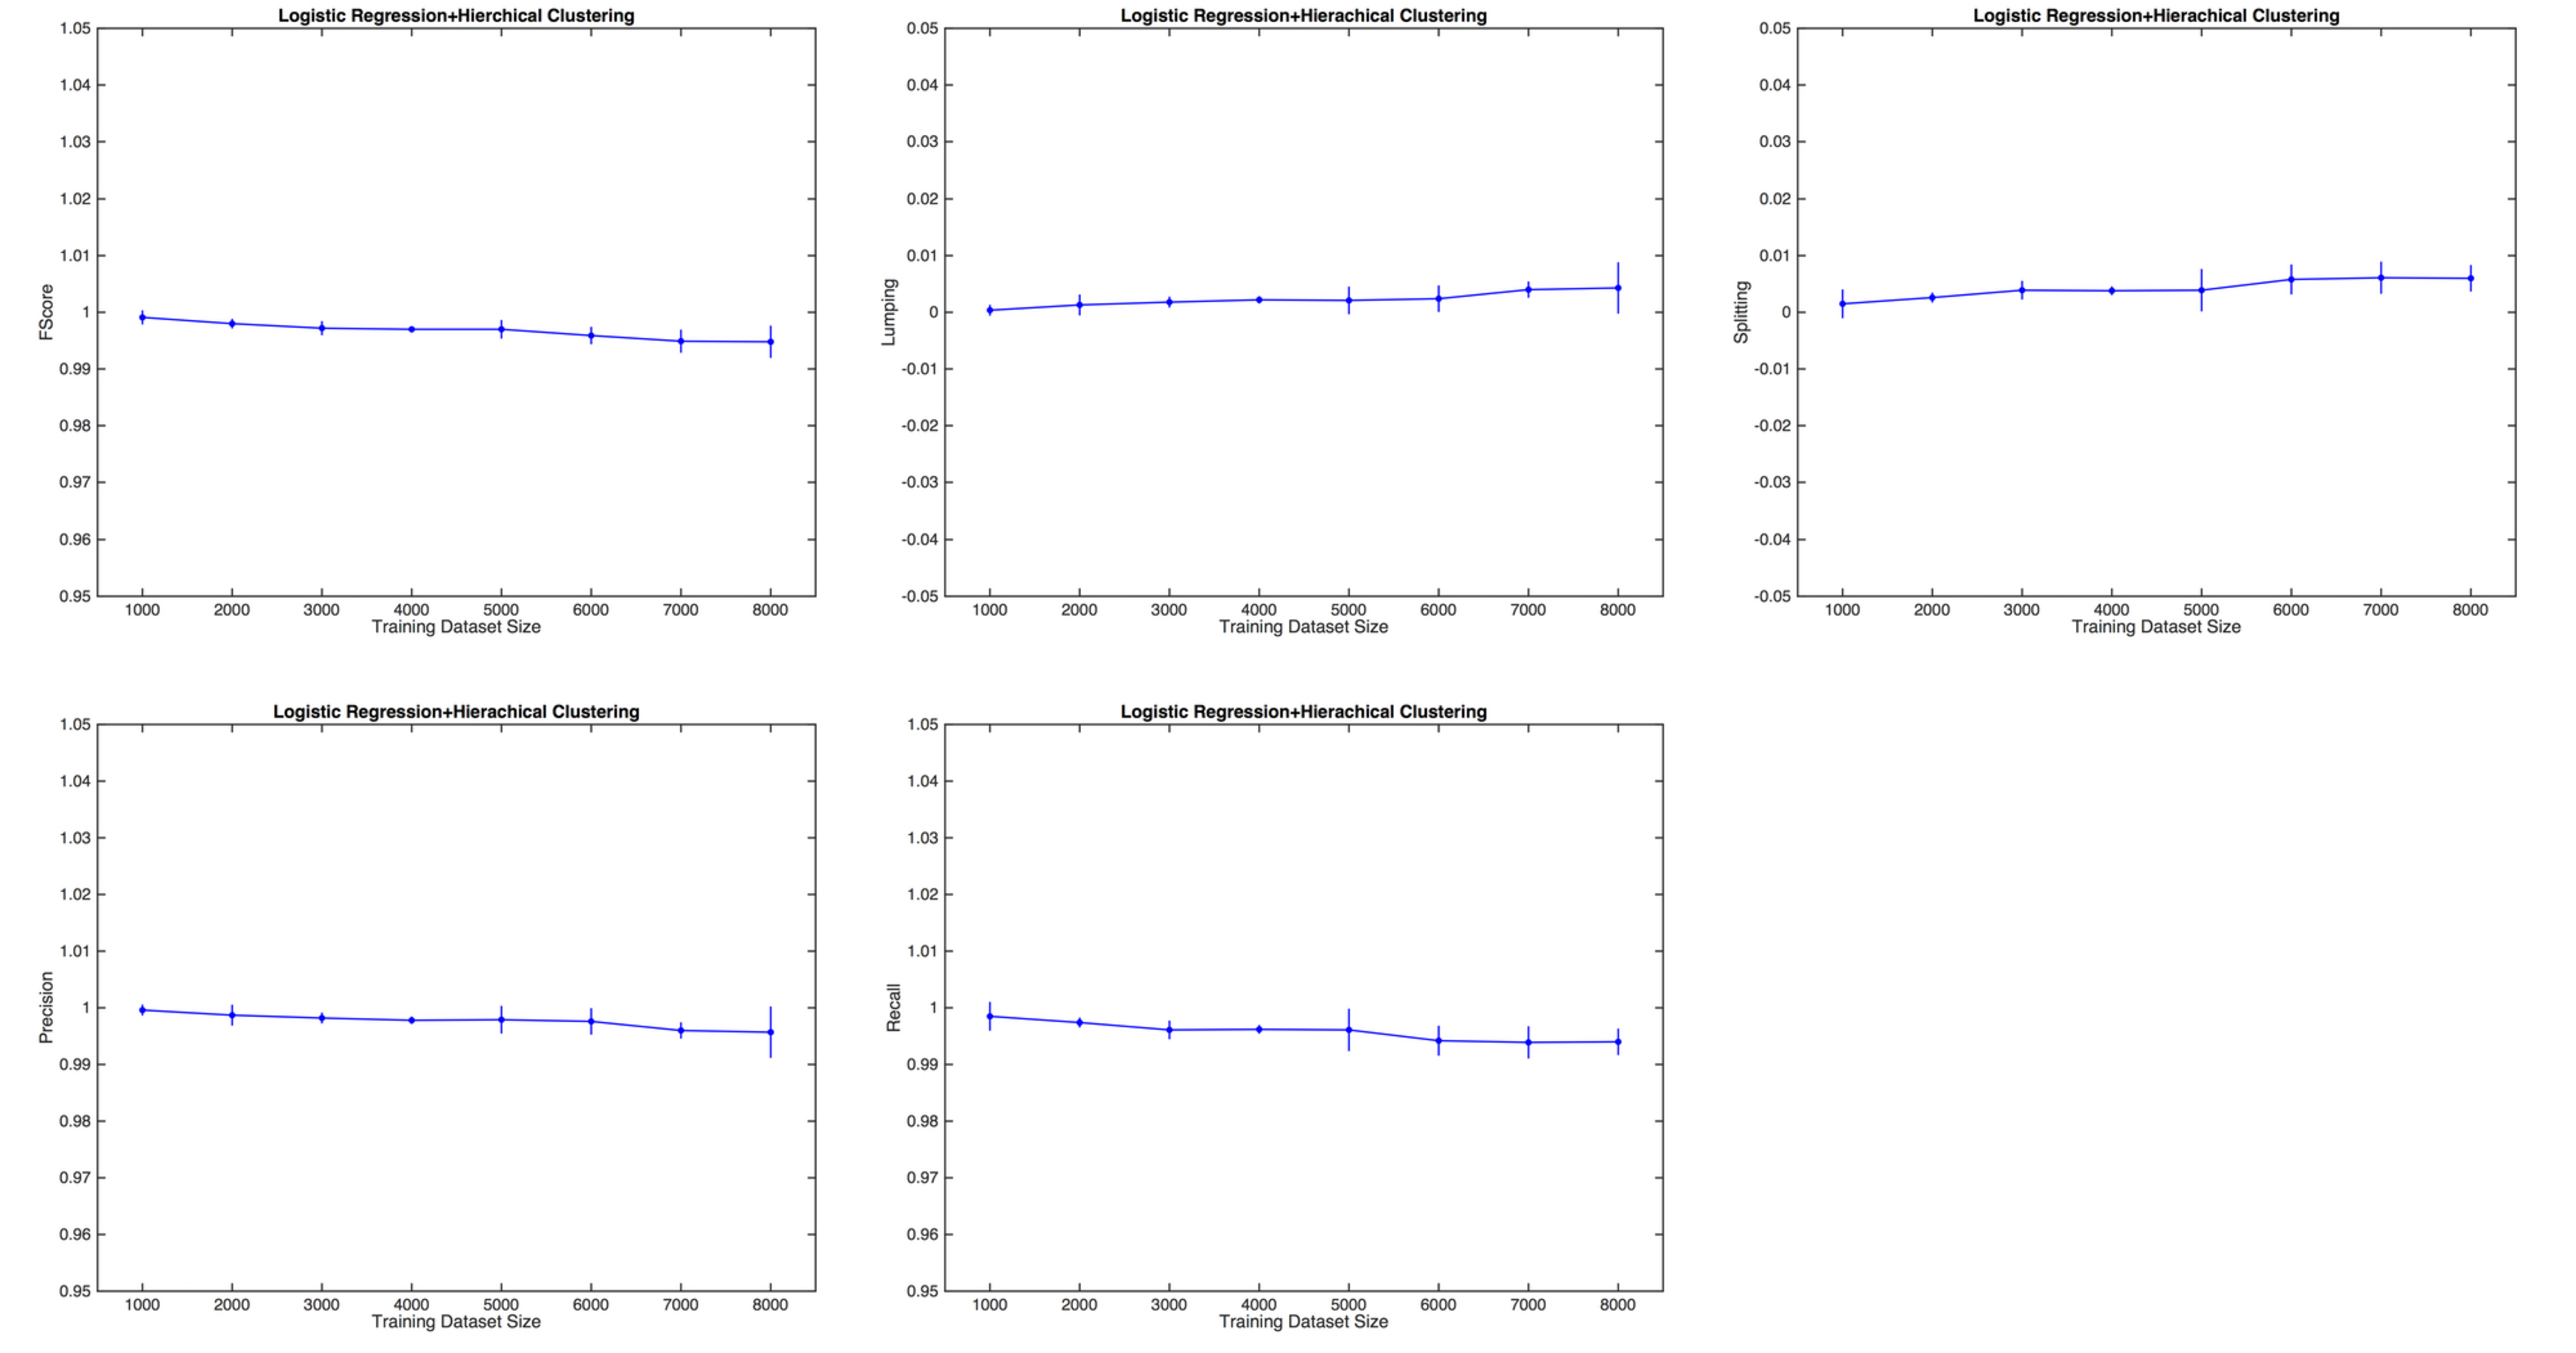
\includegraphics[scale=0.23]{CVHi.pdf}
\caption{the Cross Validation for the Hierarchical Clustering}
\end{figure}
\begin{figure} 
\centering
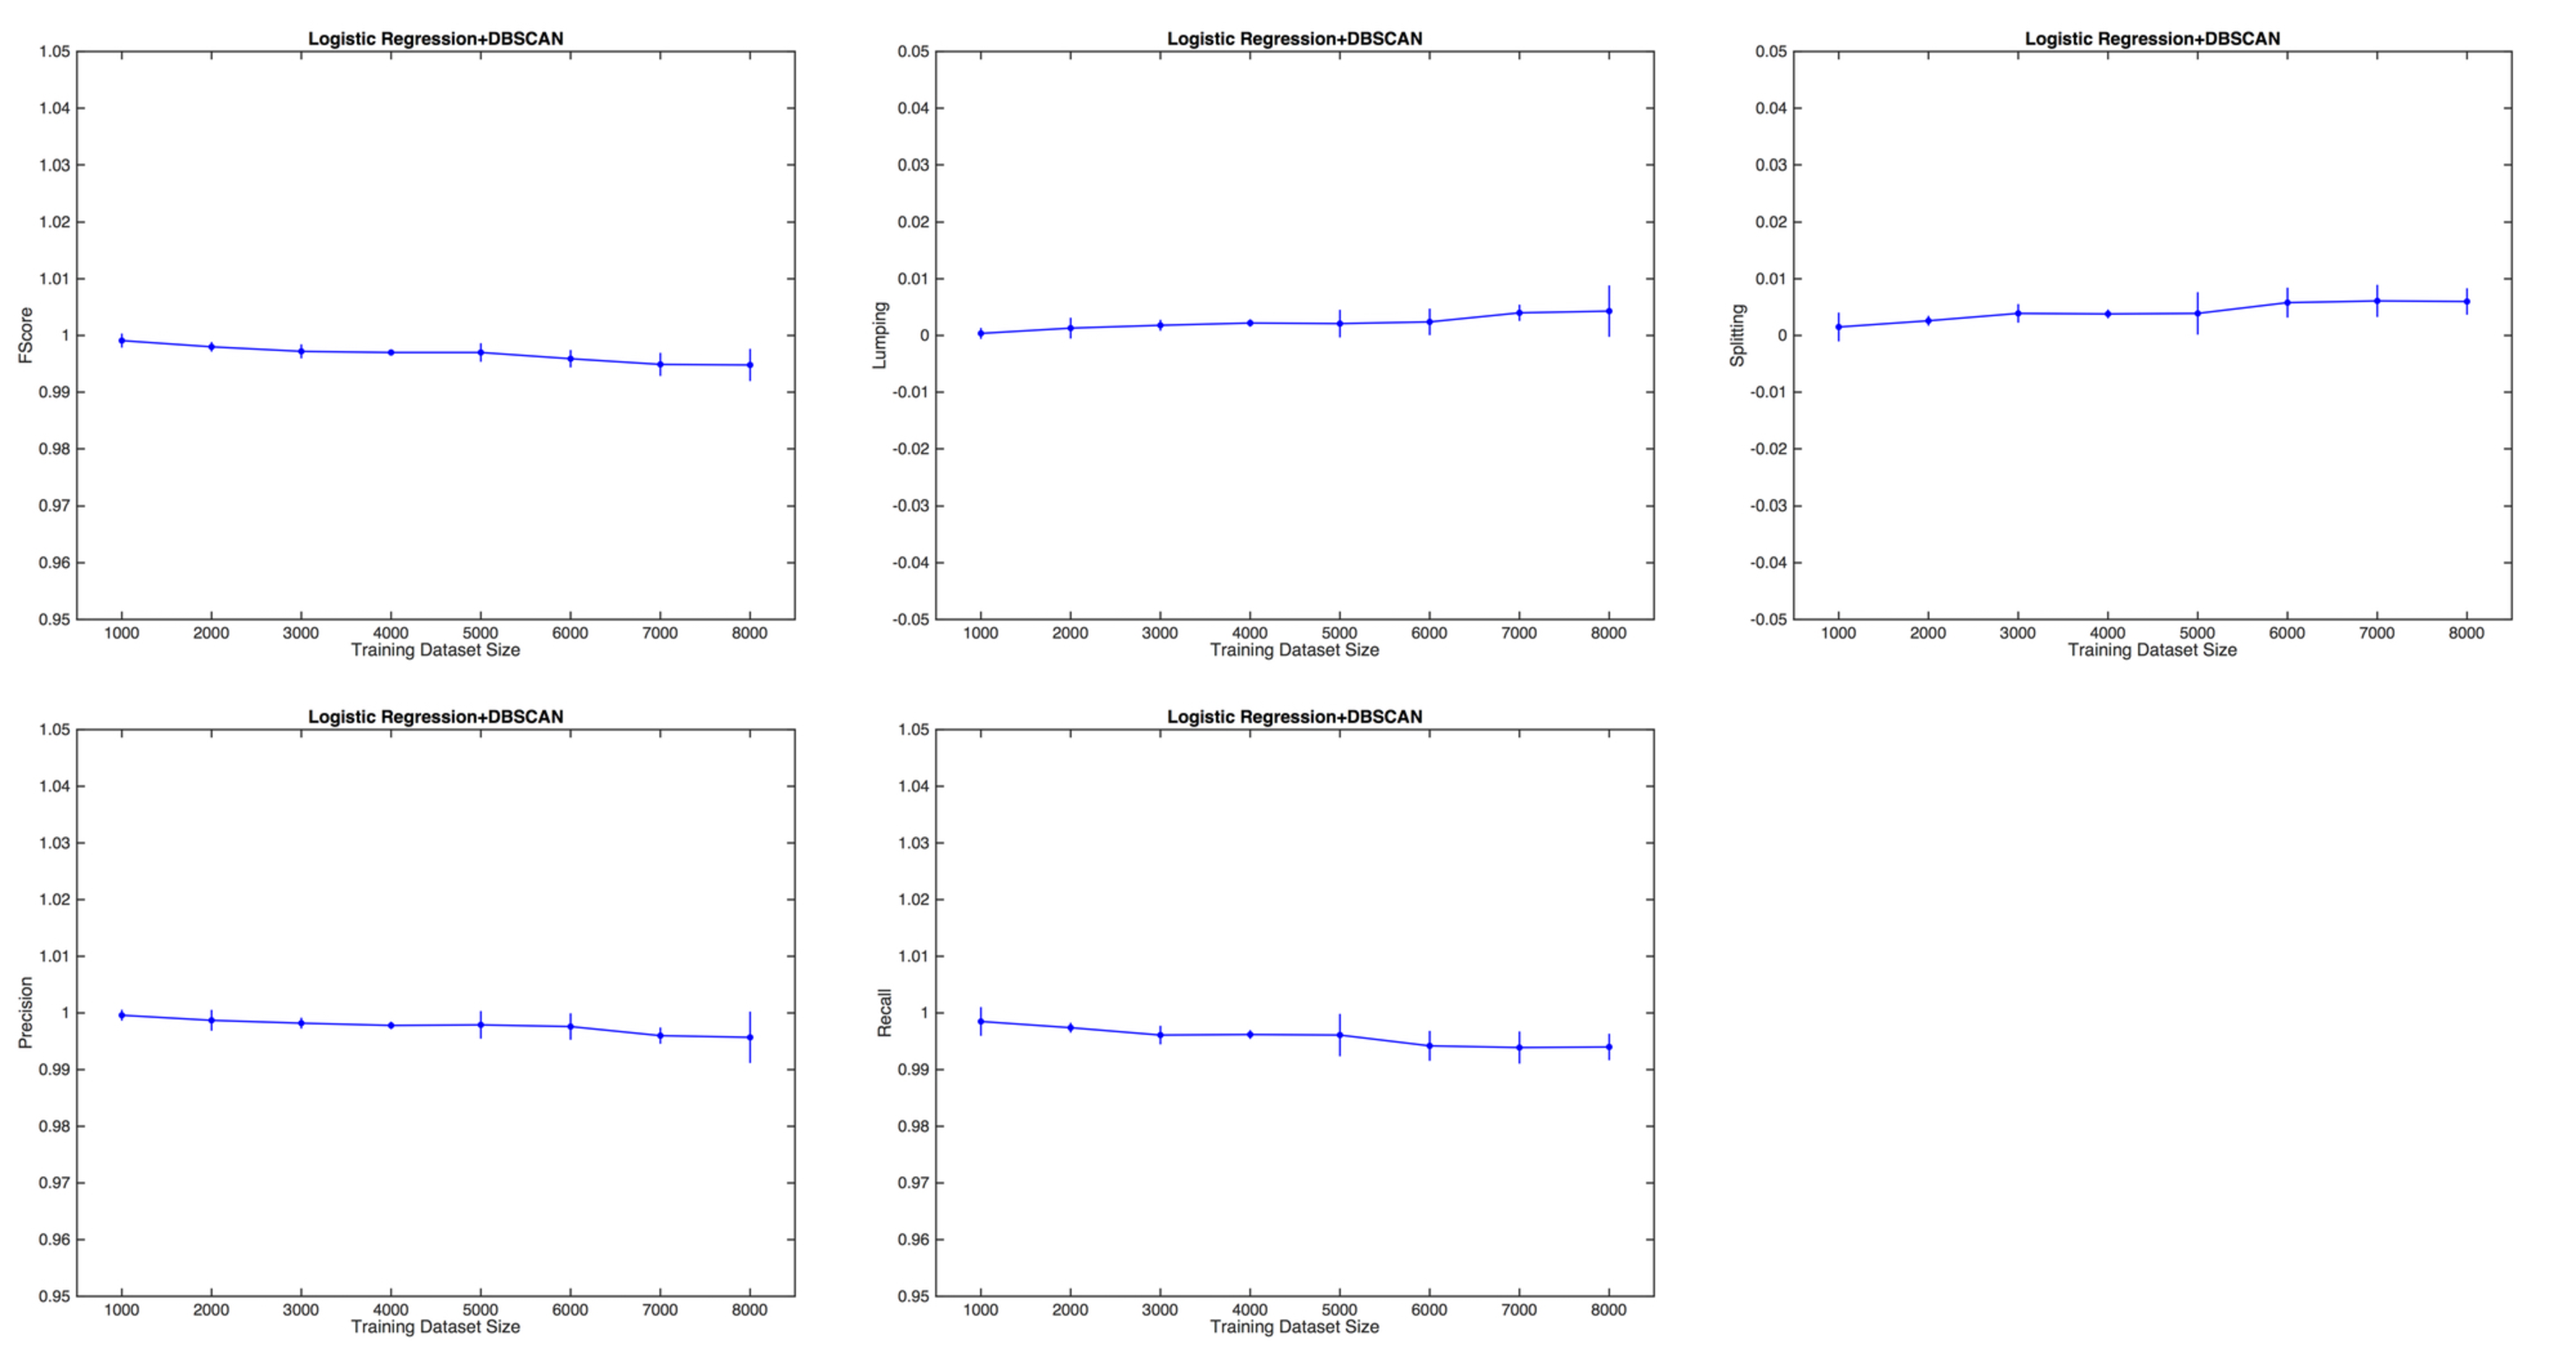
\includegraphics[scale=0.23]{CVDB.pdf}
\caption{the Cross Validation for the DBSCAN}
\end{figure}


\begin{figure}
\centering
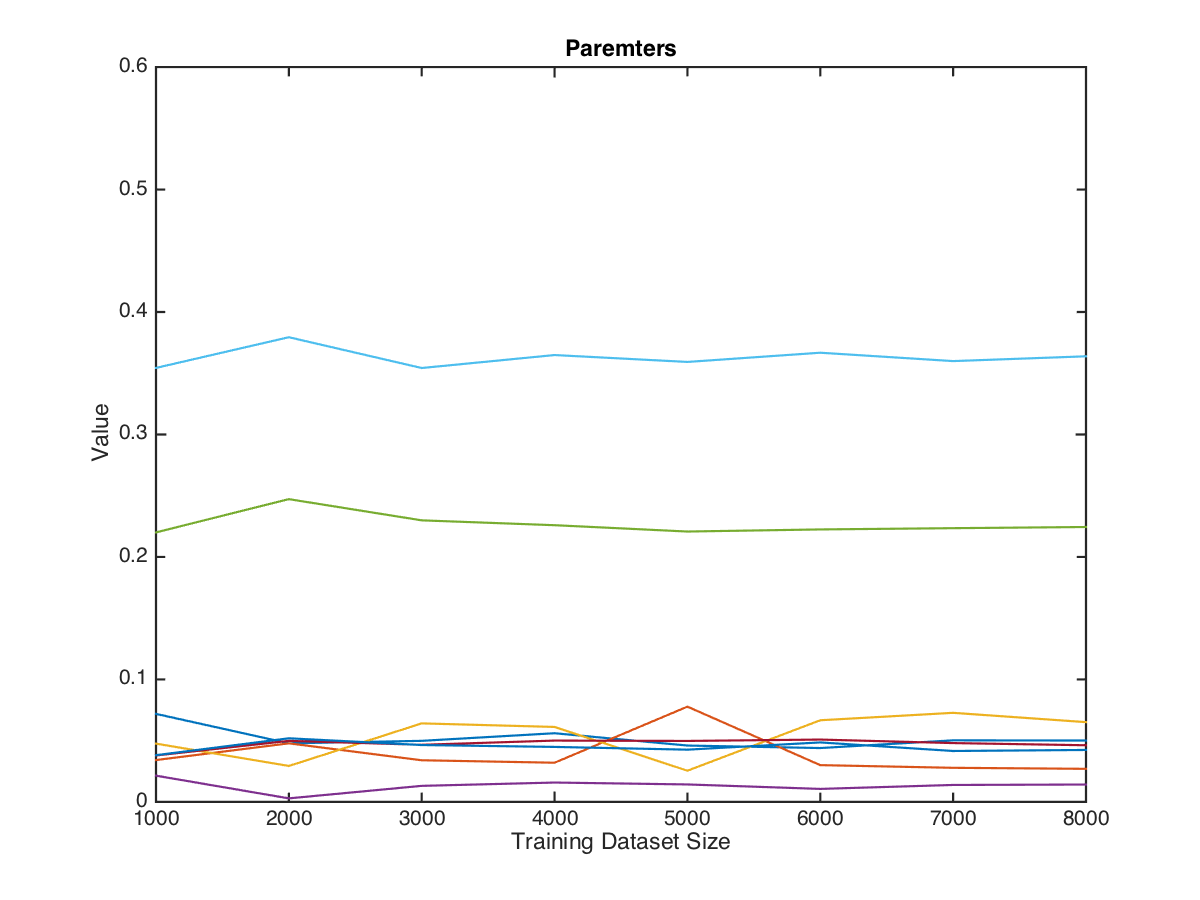
\includegraphics[scale=0.5]{parameters.png}
\caption{Parameters Values}
\end{figure}


The figure 5.3 shows the normalized parameters' values generated by the logistic regression with respect to different sizes of the training datasets. From the plot, the normalized parameter values  fluctuates when the size of the dataset changes. The changes are less than 0.1. The reason is that the subset is randomly chosen from the training dataset. Sometimes the subset of the training dataset is biased. When the size of the subset is larger than 6000, the fluctuation of the parameters decreases. From the experiments, the training dataset size should be larger than 6000 in order to get a stable result.

\subsection{the Transitivity Effect}
The hierarchical clustering has three methods to calculate the cluster similarity and the DBSCAN can changes the minPts to affect the clustering result. They affect the clustering result by changing the transitivity of the inventor identity. In the second part, the transitivity effect is evaluated. The weights and the threshold are the mean values from the results of the cross validation of the whole training dataset. An inventor-patent instance subset which contains 5000 instances  is randomly picked from the testing dataset. \newline 

For the hierarchical clustering, the three methods are evaluated by calculating the five measurements for them. The result is shown in the table 5.2. As it's explained before, the single-linkage clustering results in the chain rule while the complete-linkage clustering avoids the chain rule. The transitivity of the average-group linkage clustering is between the single-linkage clustering and the complete-linkage clustering. From the table, the single-linkage clustering has the best \emph{F-measure} and the complete-linkage clustering has the worst \emph{F-measure}.  If the transitivity of the hierarchical clustering decreases, the \emph{F-measure}, the \emph{lumping} error and the \emph{recall} of the clustering result decrease, while the \emph{splitting} error and the \emph{precision} increase. If the transitivity increases, more instances are grouped into the same cluster. As a result, the \emph{splitting} error decreases and the \emph{lumping} error increases in the contrary. For the same reason, the \emph{precision} rises and the \emph{recall} declines. Because the \emph{F-measure} is the main measurement, the single-linkage clustering shows the best performance compared to the other two methods. \newline

\begin{table}
\centering
\begin{tabular}{|c|c|c|c|c|c|}
\hline
&F1&Lumping&Splitting&Precision&Recall\\
\hline
Single Linkage& 0.99396&0.00336 &0.00870 &0.99662 &0.99130 \\
\hline
Average Group Linkage&0.99268 &0.00196 & 0.01259& 0.99802& 0.98740\\
\hline
Complete Linkage&0.98588 & 0.00112 & 0.02657 &0.99885 &0.97343 \\
\hline
\end{tabular}
\caption{the Transitivity Effect of the Hierarchical Clustering}
\end{table}
\begin{figure}
\centering
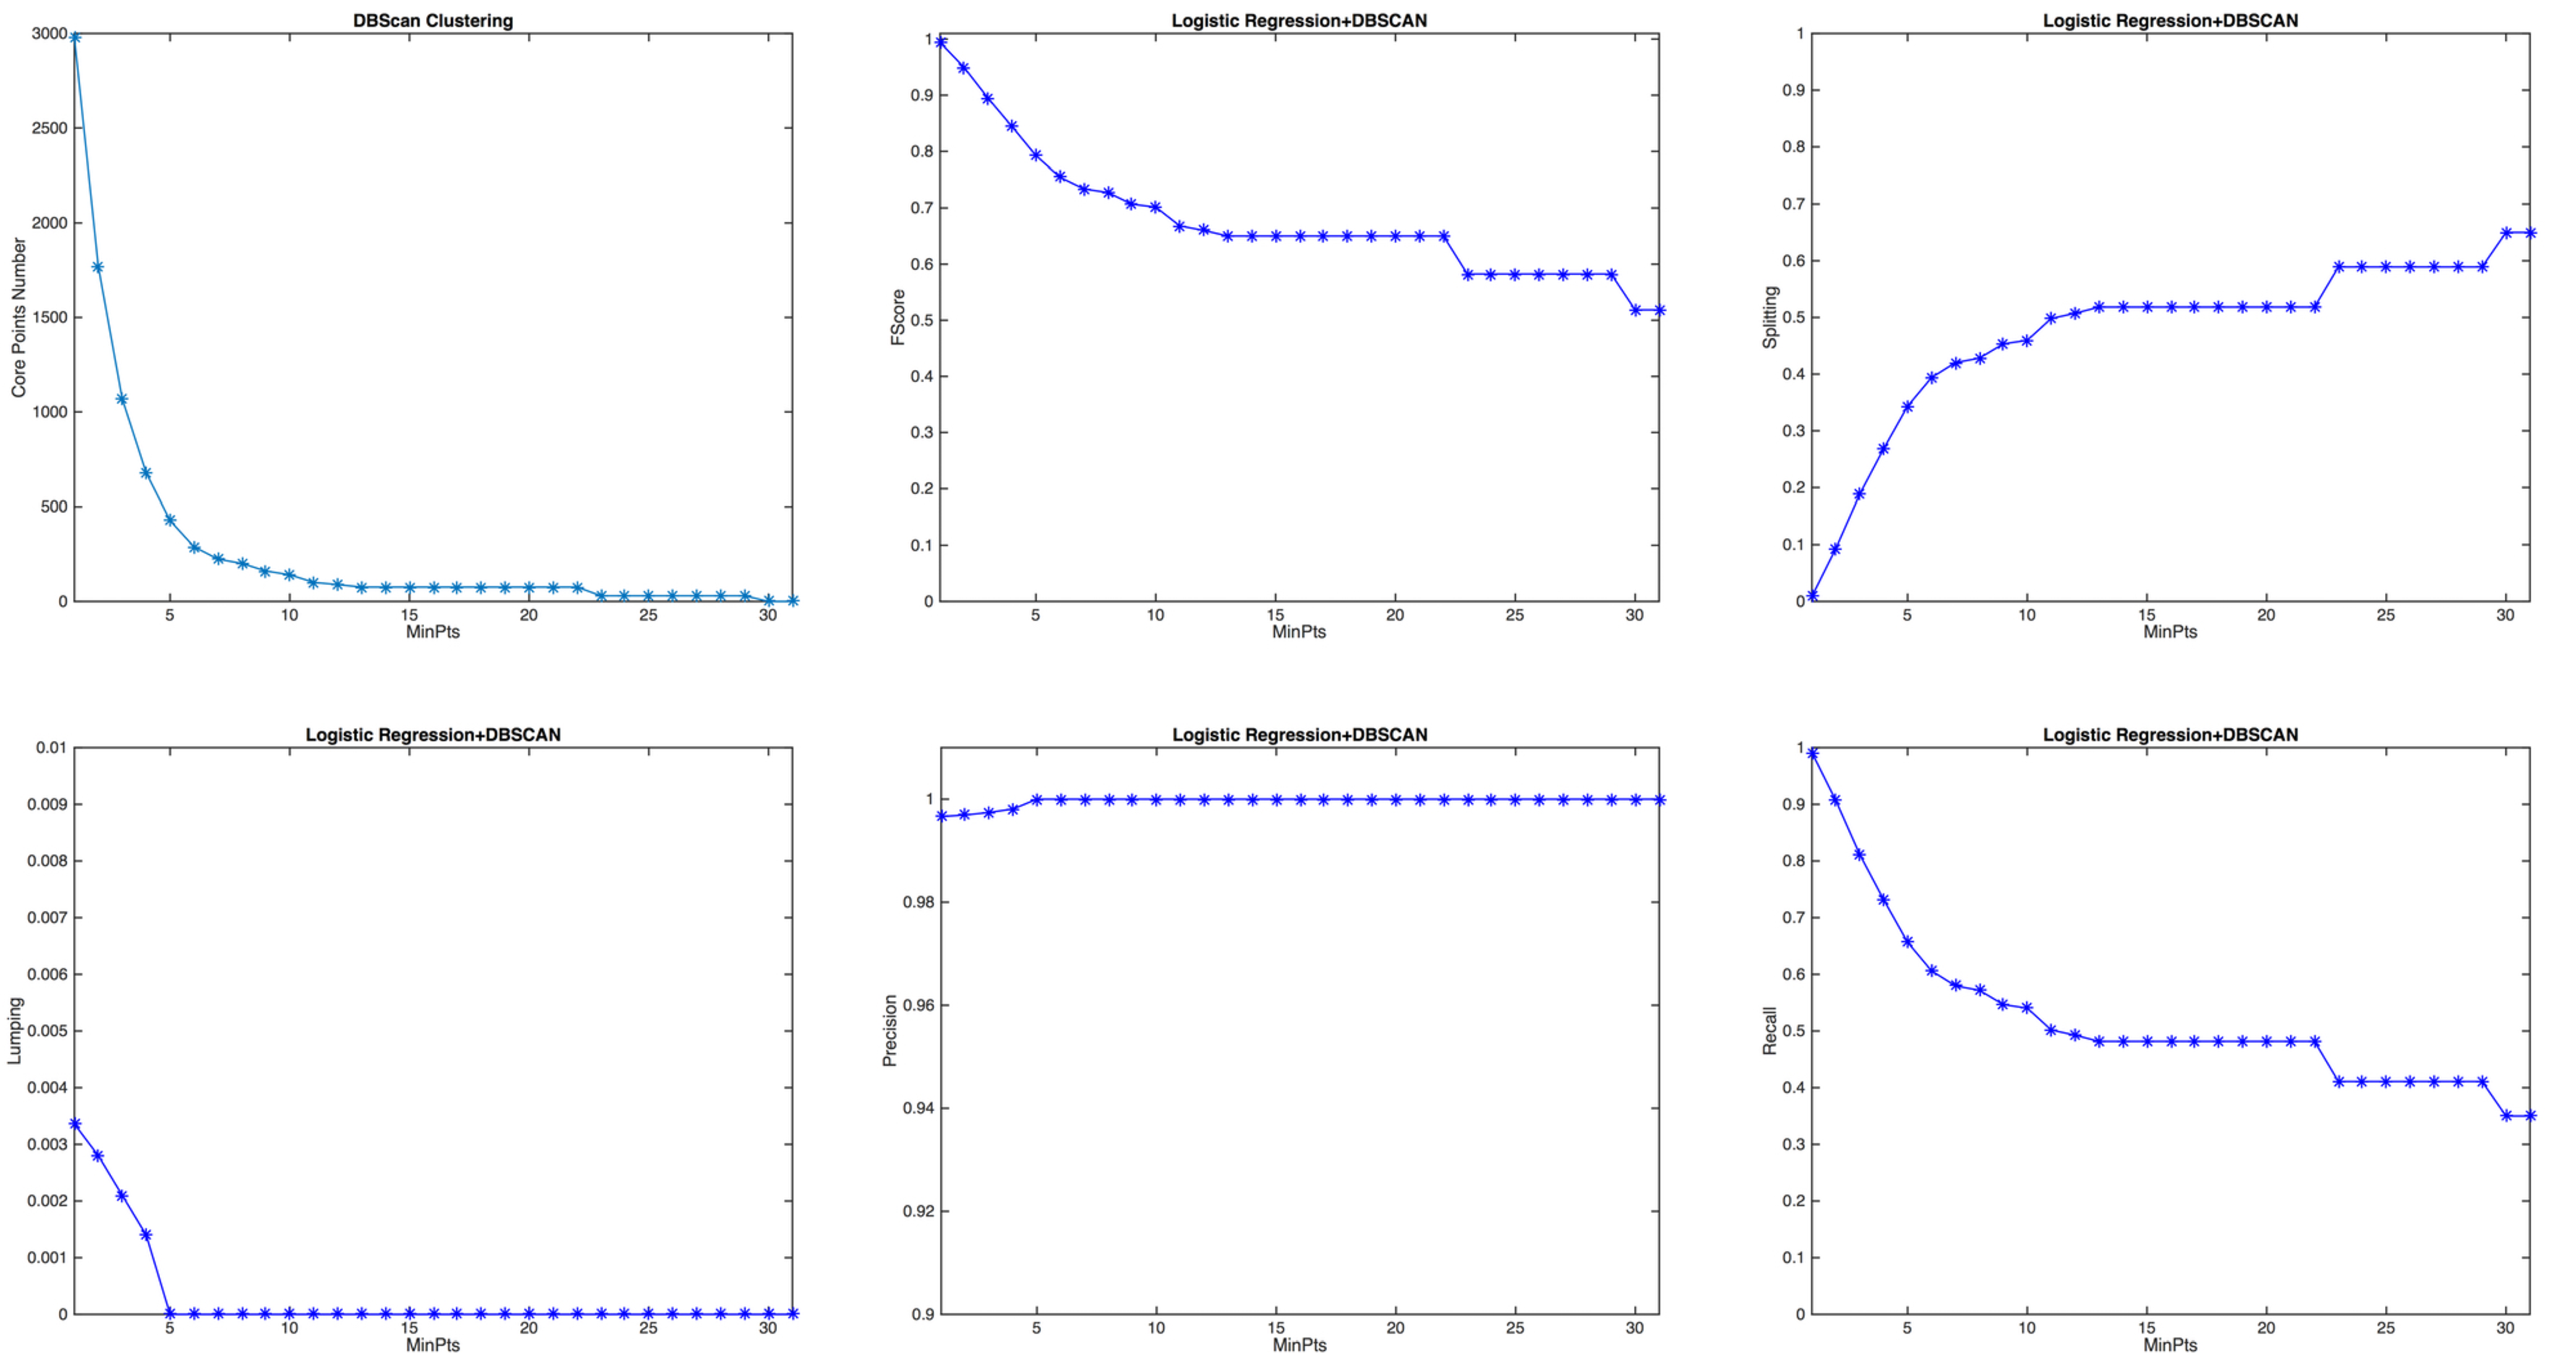
\includegraphics[scale=0.2]{DBSCANT.pdf}
\caption{the DBSCAN Performance with respect to minPts}
\end{figure}

For DBSCAN, the radius is the threshold generated by the logistic regression. The minPts decides which inventor-patent instances are core objects for the DBSCAN. The instances grouped into a cluster should be similar to at least one core object in the cluster. The minPts value affects the number of the core objects. The core objects affect the clustering result. From the figure 5.4, the number of the core objects decreases as the value of MinPts incrases. The \emph{precision} error increases and the \emph{lumping} error decreases. After the MinPts is larger than 5, the \emph{precision} and the \emph{lumping} error remain the same as 1 and 0. It means that after the MinPts reaches 5, the instances from the same clusters are all from the same inventors. The \emph{splitting} error keeps increasing and the \emph{recall} keeps decreasing as the MinPts increases which means more and more instances from the same inventors are considered to be from different inventors. When the MinPts reaches 30, the number of the core objects becomes 0. Each instance is put into a single cluster. The clustering result will not change any more. From the plot, the DBSCAN with the value 1 for MinPts shows the best performance which has the best \emph{F-measure}. In conclusion, from the transitivity evaluation, the transitivity is proved to be helpful for improving the accuracy of the inventor identification.

\subsection{the Clustering for Testing Datasets}
\begin{table}
\centering
\begin{tabular}{|c|c|c|c|c|}
\hline
F-measure&Lumping Error&Splitting Error&Precision&Recall\\
\hline
0.99151&0.01497&0.00212&0.98522&0.99788\\
\hline
\end{tabular}
\caption{the Clustering Evaluation for the Whole Testing Dataset}
\end{table}

From the second part of the evaluation, the single-linkage clustering and the DBSCAN with MinPts 1 show the best performances. Therefore, they are chosen for the evaluation of the whole testing dataset. The values for the weights and threshold keeps the same as the second part. For the third part, subsets are randomly chosen from the testing dataset with different sizes to test the clustering performance by calculating the five measurements. The size of the subset is from 2000 to 24495 and the increment is 2000.\newline 

The figure 5.5 and the figure 5.6 show the performance of the DBSCAN and the hierarchical clustering separately based on the five measurements. As it is explained before, setting MinPts as 1 makes the DBSCAN clustering result same as the hierarchical clustering by using the single-linkage clustering method. The values of the \emph{F-measure}, the \emph{precision} and the \emph{recall} are around 0.99. The \emph{lumping} error and \emph{splitting} error are less than 0.02. The subset with the size 2000 has the worst \emph{F-measure} as 0.988 and the largest \emph{splitting} error as 0.0159. The table 5.3 shows the five measurements for the whole testing dataset.  The best \emph{F-measure} which the approaches of the PatentsView Inventor Disambiguation Workshop have on the E\&S dataset is 0.983. As the whole E\&S dataset is not provided, it's difficult to compare the performance of my approach with that of the approaches of the workshop. However, the \emph{F-measure} of my approach on the incomplete  E\&S dataset is 0.99151. Therefore, my approach is promising to have a better performance.

\begin{figure}
\centering
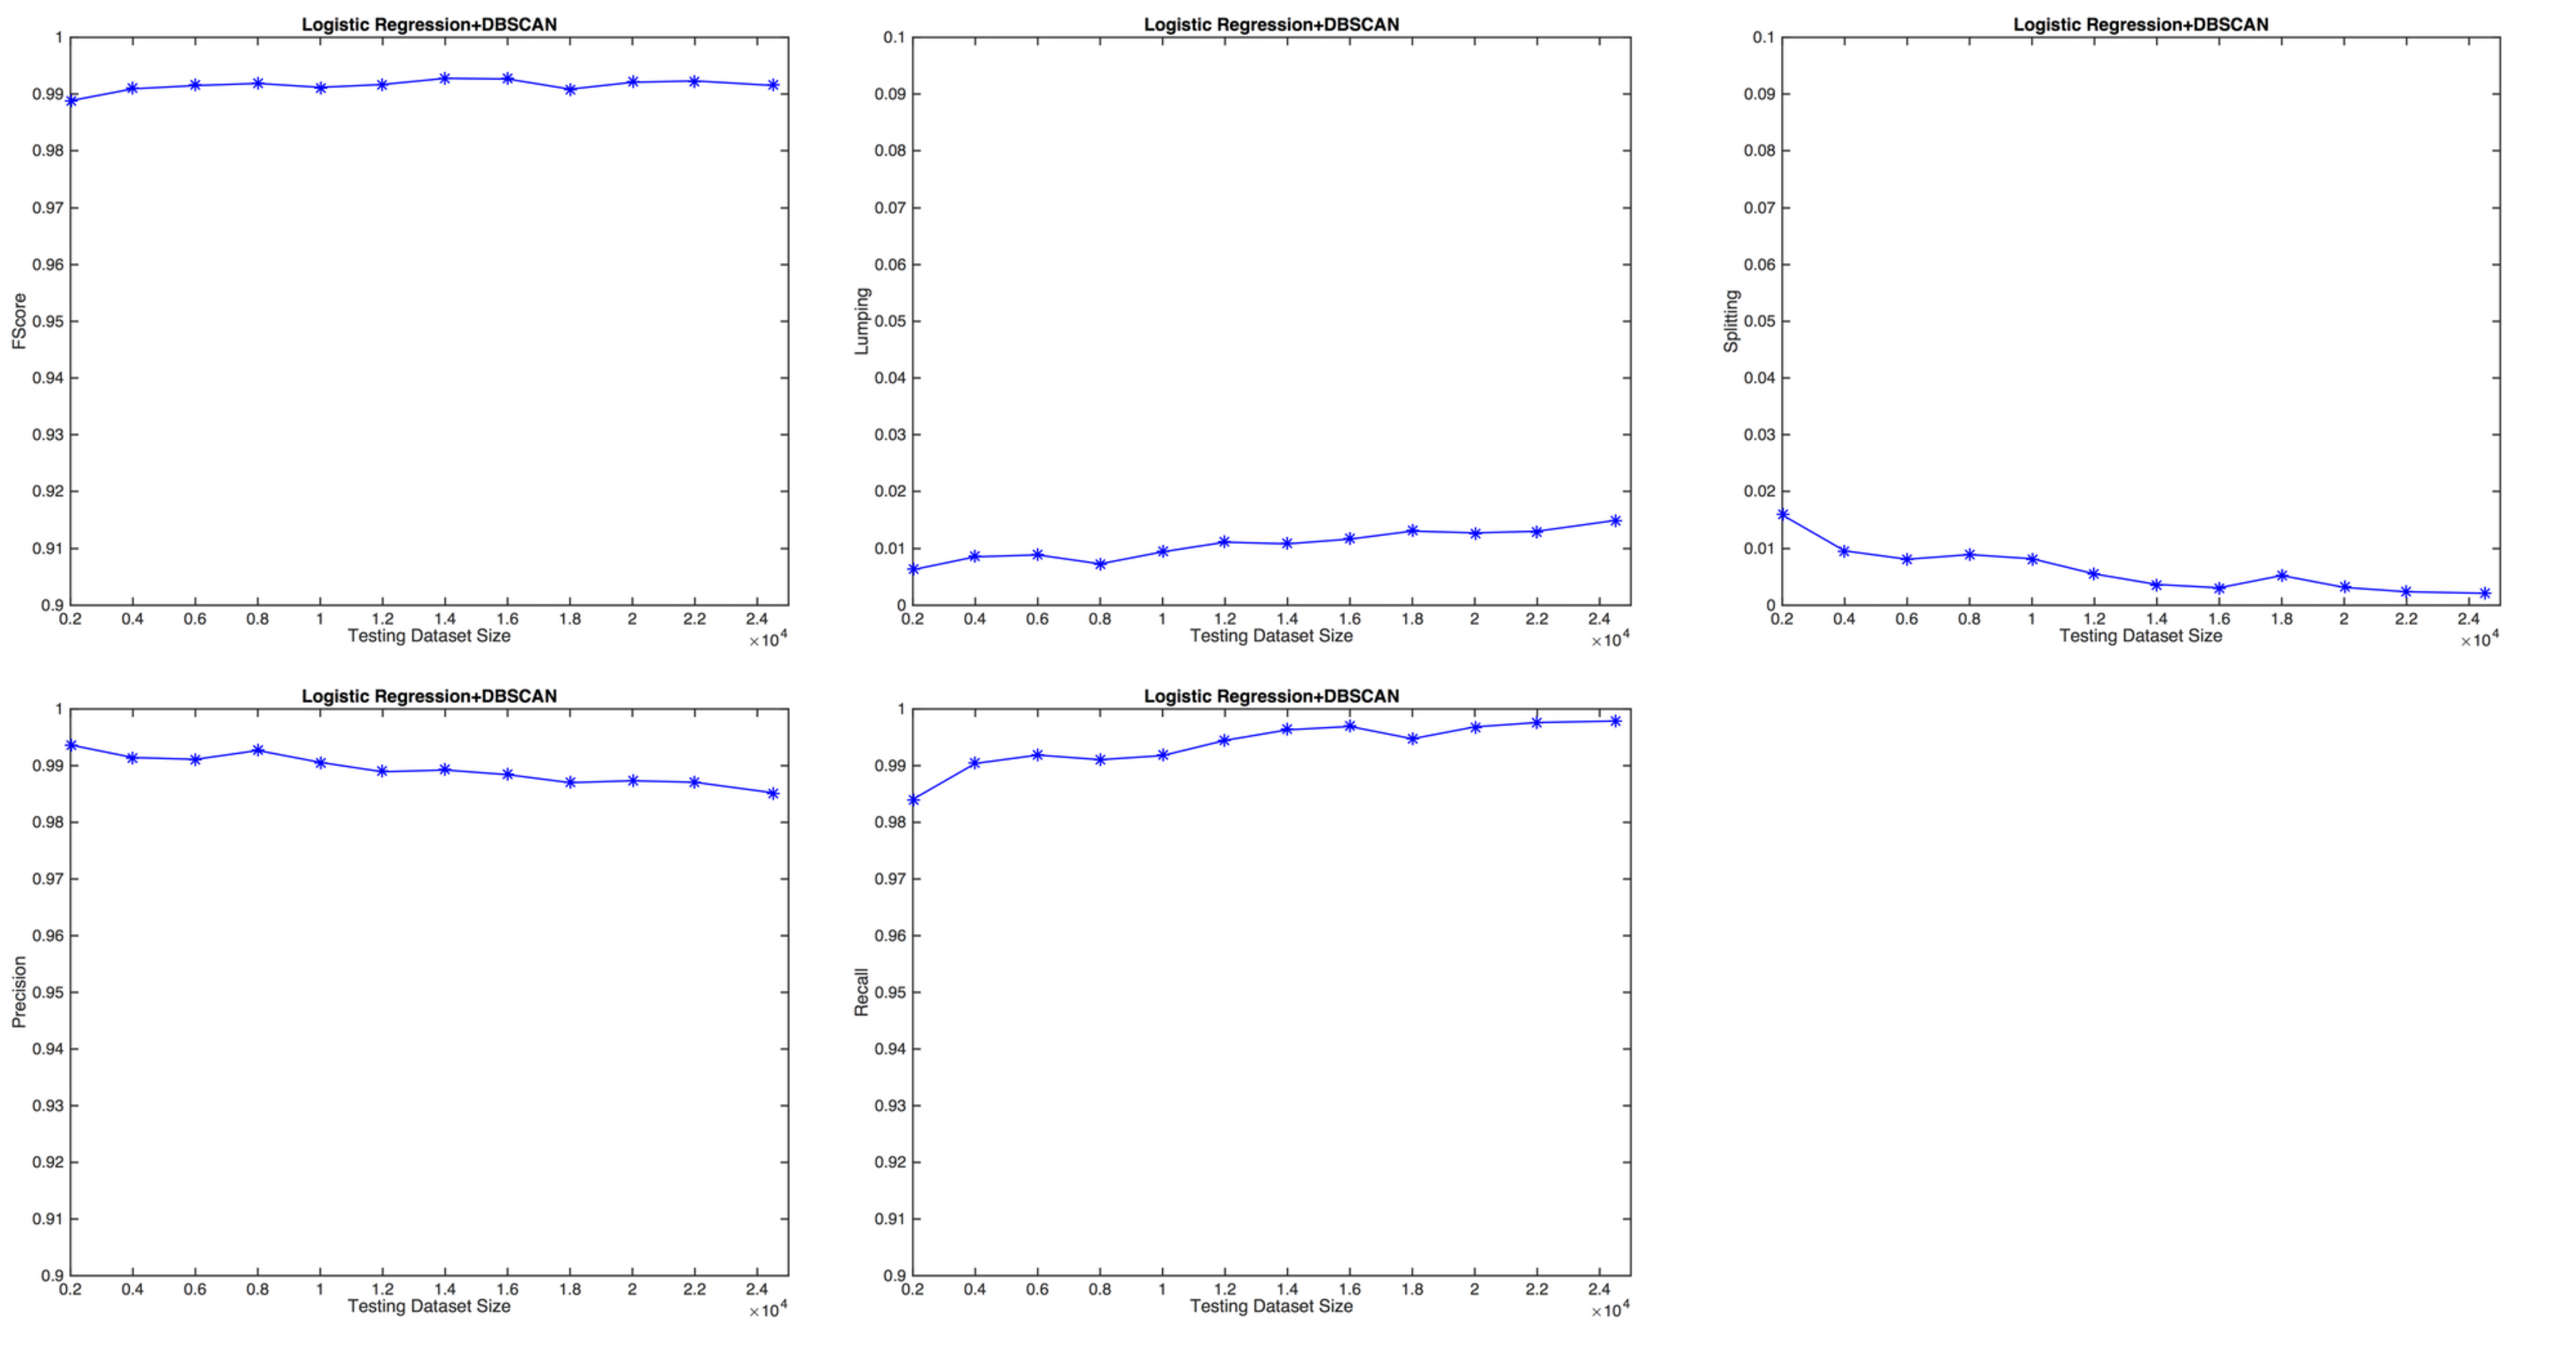
\includegraphics[scale=0.23]{DBTest.pdf}
\caption{the DBSCAN Evaluation for the Testing Dataset}
\end{figure}
\begin{figure}
\centering
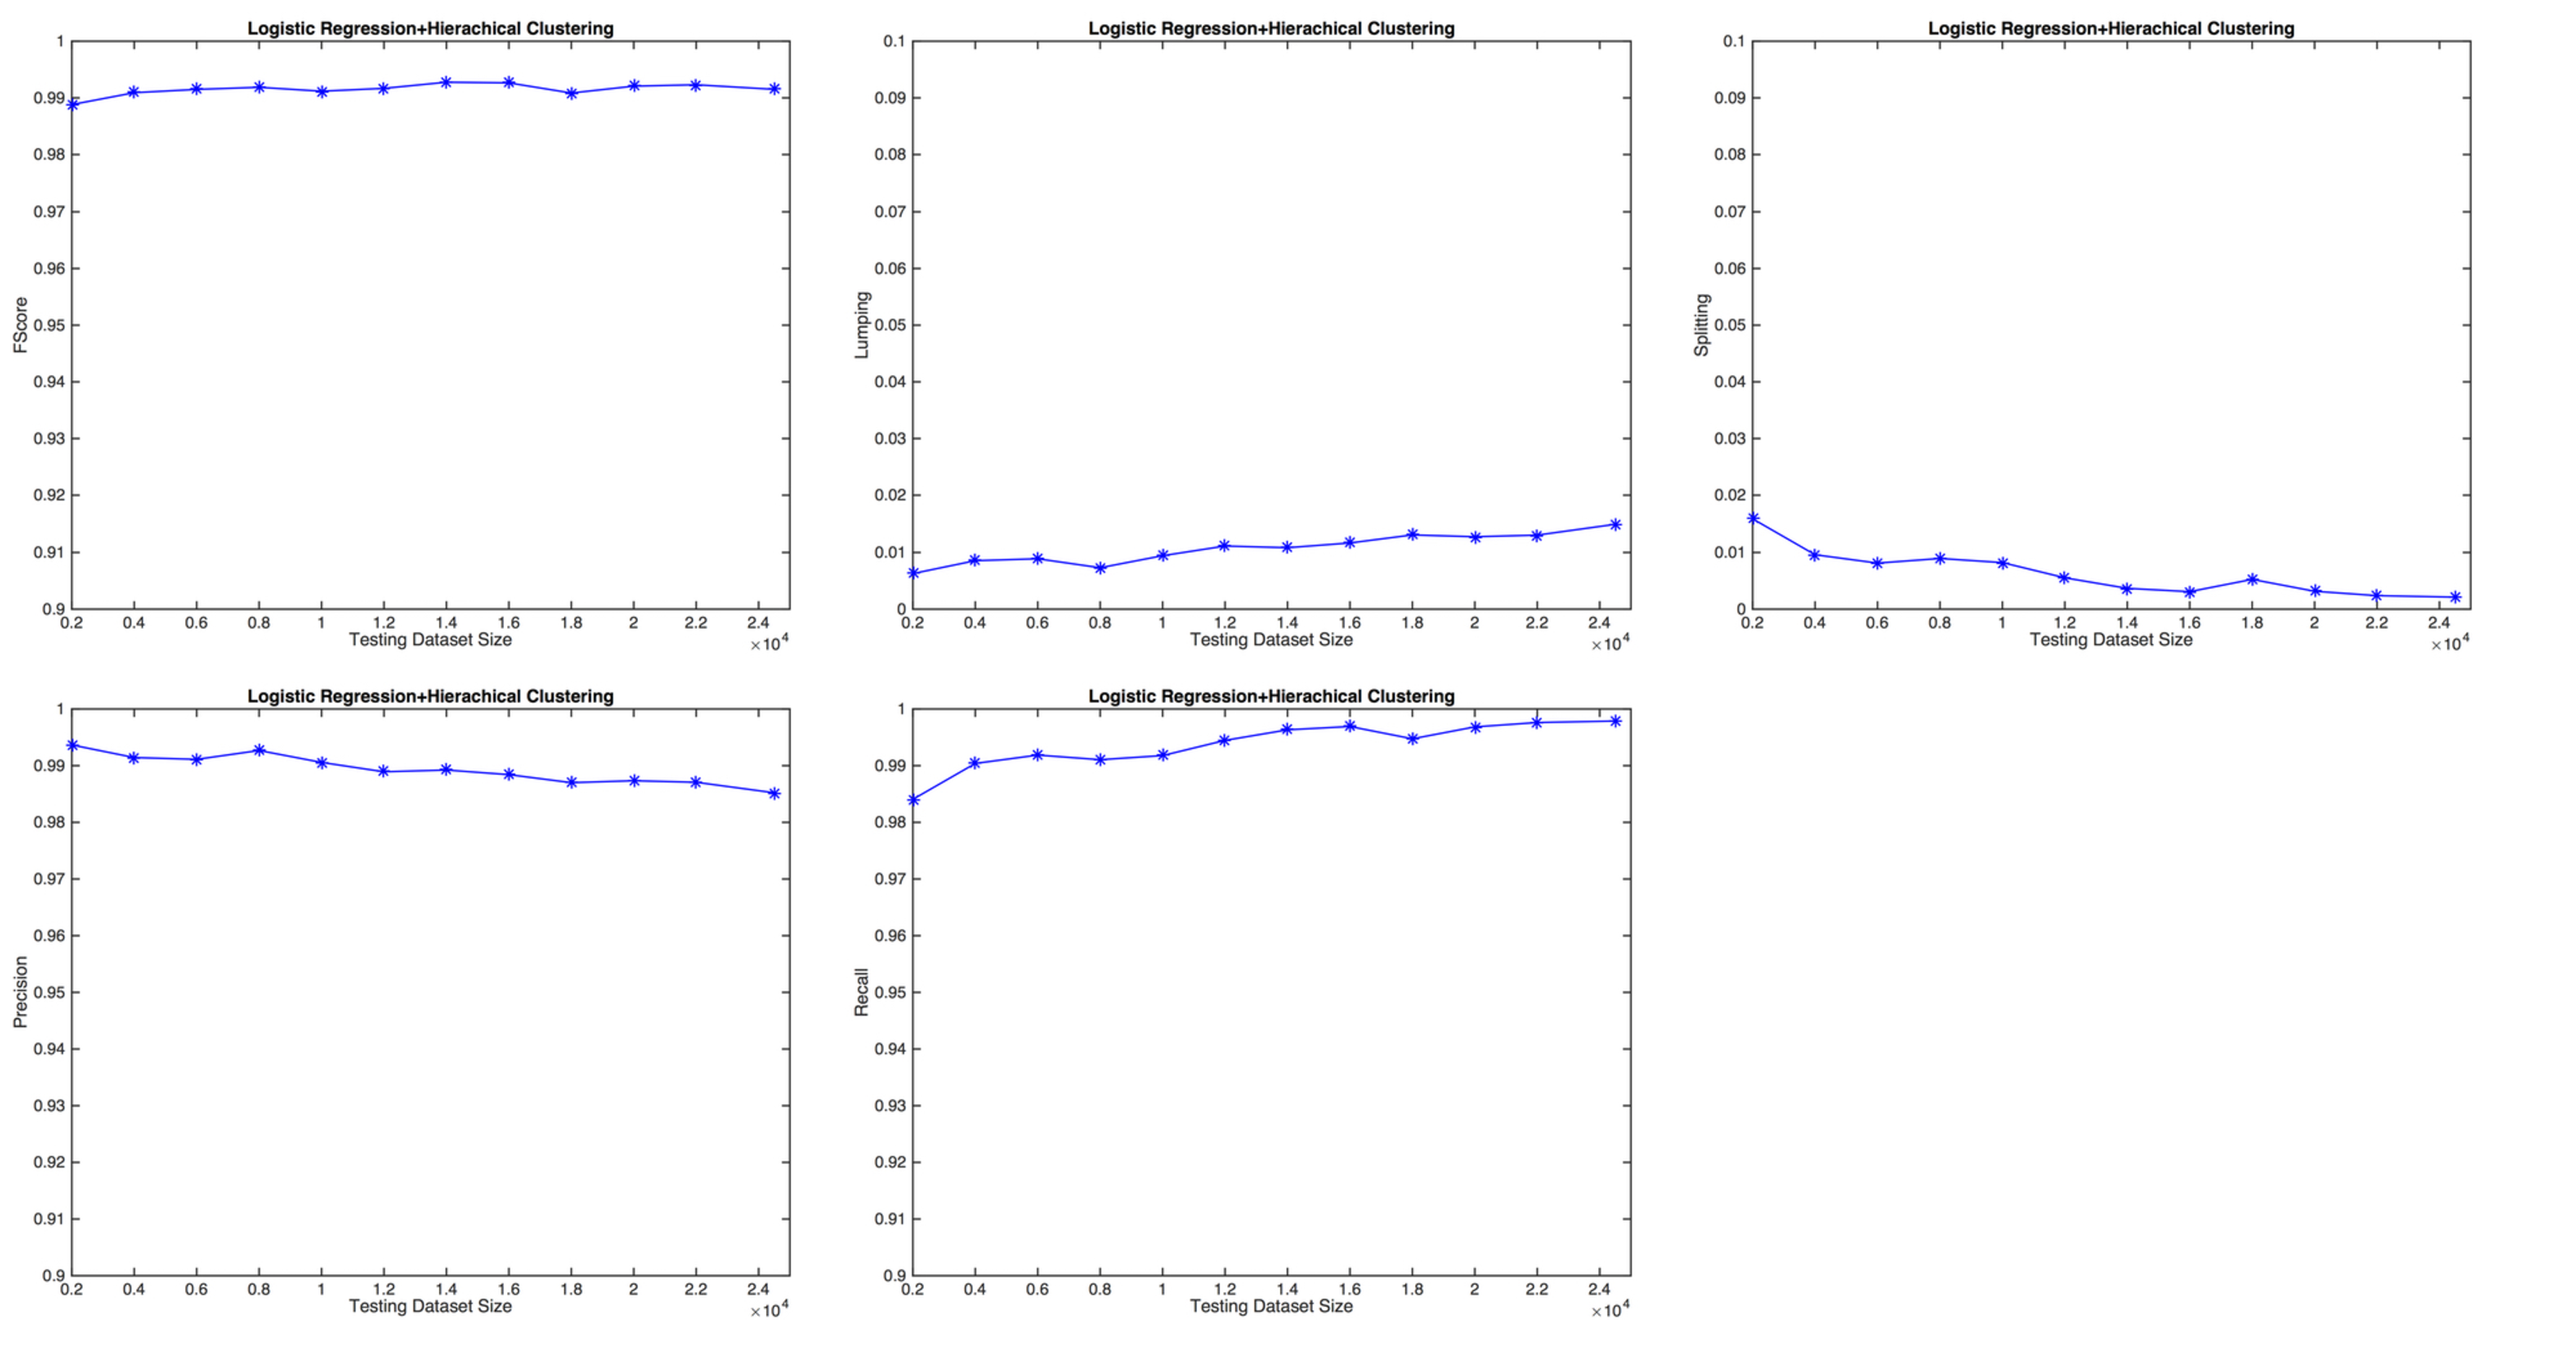
\includegraphics[scale=0.23]{HITest.pdf}
\caption{the Hierachical Clustering Evaluation for the Testing Dataset}
\end{figure}
   

\subsection{the Comparison with the Flemming's approach}
Flemming uses a benchmark dataset to test the performance of his approach. The benchmark dataset contains 95 US inventors and 1332 inventor-patent instances.  Flemming's approach uses inventor name blocking techniques.  With different blocking rules, the approach gives two different results for the inventor identification which are named as \emph{Lower-bound} and \emph{Upper-bound}. In the fourth part of the evaluation, my approach is used to do an inventor identification for the benchmark dataset and compare my approach's result with the Flemming's. \newline
\begin{table}
\scriptsize
\begin{tabular}{|c|c|c|c|}
\hline
&F-Measuremen&Lumping Error&Splitting Error\\
\hline

\emph{Upper-Bound} (Flemming)&0.9744 &0.0150&0.0357\\

\hline

\emph{Lower-Bound}(Flemming)&0. 9764& 0.0150& 0.0319\\
\hline
Logistic Regression + (DBSCAN ,Hierarchical Clsutering) & 1.0 &0.0&0.0\\
\hline
\end{tabular}
\caption{the Comparison with Flemming's Approach}
\end{table}

The table 5.4 shows the \emph{F-measure}, the \emph{lumping} error and the \emph{splitting} error for the Flemming's \emph{upper bound} and \emph{lower bound} and my approach. All the inventors have been identified correctly by using my approach. The performance of my approach is better than the Flemming's for the benchmark dataset. 

\subsection{the Patent-publication Matching}
In the fifth part of the evaluation, the improvement of the accuracy by using the patent-publication matching is evaluated. The subset which contains 3604 inventor-patent instances from the intersection set is used. All these patents of the inventor-patent instances are from the bio-medical field in order to use the Europe PMC database.  The table 5.4 shows the evaluation result. \newline
\begin{table} 
\scriptsize
\begin{tabular}{|c|c|c|c|c|c|}
\hline
&F-measure&Lumping Error&Splitting Error&Precision&Recall\\
\hline
Before the patent-publication matching&0.9992&7.4056e-4&8.6398e-4&0.9993 &0.9991\\
\hline
After the patent-publication matching&0.9992&7.4056e-4&8.6398e-4&0.9993 &0.9991 \\
\hline
\end{tabular}
\caption{the Patent-publication Matching}
\end{table}

From the table 5.5, it shows that the patent-publication matching doesn't help to improve the accuracy of the clustering result. There are two reasons for that. First, the clustering result already shows an almost correct inventor identification. An improvement for that is difficult. Second, the publication doesn't provide complete information for the author ID, the abstract and the affiliation and it increases the difficulty for the accuracy improvement.
\newpage
\thispagestyle{empty}
\rule{0cm}{5cm}